\newpage
\section{Исследование и построение решения задачи}
\label{research}
% В разделе «Исследование и построение решения задачи» должна быть проведена
% декомпозиция исходной задачи на последовательность подзадач, которые нужно
% решить для получения решения исходной задачи, приведены обосновании всех
% принимаемых решений. Например, если принимается решение о создании некоторого
% программного средства, то необходимо показать, что не существует средства,
% обладающего нужными характеристиками. Исключение составляет случай, когда
% такое средство создается в учебных целях. Обоснование может быть дано одним
% из следующих способов:
% 1.Экспертный: приводятся высказывания, мнения авторитетных специалистов, с
% указанием ссылок на источники, где оно сформулировано;
% 2.Дедуктивный: яркий пример математика - есть система аксиом и правил вывода.
% Если ты сумел показать, как вывести свое утверждение из аксиом с помощью
% правил вывода, то все обосновано.
% 3.Естественнонаучный: выдвигается
% гипотеза (то, что обосновываем) и проводится серия экспериментов, на основании
% обработки результатов этих экспериментов гипотеза либо подтверждается, либо нет
% 4. Инженерно-практический:  хорош когда в качестве утверждения выступает некий
% принцип или система, работоспособность которого мы хотим обосновать, тогда
% экспериментальная реализация может выступать в качестве обоснования..

Для того чтобы применить метод опорных векторов к задаче фильтрации спама,
необходимо научиться представлять письма в виде, пригодом для применения
этого метода - в виде вектора.
Кроме того нам необходимо построить многопровильную систему, а для этого
классифицируемый вектор должен содержать какую-то информацию о пользователе.

\subsection{Выделение токенов}
Под \textbf{токенами} мы будем понимать последовательности символов, на которые мы разбиваем исходный текст. В некотором смысле токен - это аналог слова. Выделить слова из текста зачастую бывает затруднительно, кроме того зачастую смысловую нагрузку несет лишь часть слова, а иногда напротив лишь последовательность слов. Для разбиения текста на токены существует несколько способов:
\begin{itemize}
\item \textbf{Разбиение до пробельных символов или знаков препинания}. В этом случае токен получается практически полным аналогом слова. Например текст ``Как хорошо, замечательно жить в этом мире!'' разобьется на следующие токены:
 ``Как'' , ``хорошо'', ``замечательно'', ``жить'', ``в'', ``этом'' и ``мире''.

 \item \textbf{Выделенеие n-грамм}. В этом случае из текста выделяются все цепочки содержащие ровно n символов. Например при n=6 фраза ``hello, world'' породит следующие 6-граммы: ``hello,'', ``ello, '', ``llo, w'', ``lo, wo'', ``o, wor'', ``, worl'' и `` world''.

 \item \textbf{Выделение цепочек}. Использование в качестве токенов цепочек из нескольких слов. При этом в качестве токенов выделяются как сами слова, так и последовательности из нескольких подряд идущих слов. Например ``free viagra'' породит токены ``free'', ``viagra'' и ``free viagra''.
\item {Выделение частичных цепочек}. Этот алгоритм рассматривает окна из нескольких слов, и генерирует цеочки состоящие из некоторых(необязательно идущих подряд) слов этого окна. Например, из  текста ``the quick brown fox jumped'' при размере окна 4 будут сгенерированы такие токены как ``the quick brown *'', ``quick * * jumped'', ``* * * jumped'' и другие.

\item {Выделение биграмм}. Алгоритм похож на использование частичных цепочек, однако генерирует только те цепочки, в которых содержится ровно два слова. Для предыдущего примера алгоритм сгенерирует цепочки ``the quick * *'' ``* * brown jumped'', ``the * * fox''  и другие.
\end{itemize}

Проведенные эксперименты показали, что способ выделения токенов из письма не оказывает существенного влияния н а качество классификации, поэтому для решения задачи был выбран используемый в системе dspam по-умолчанию способ выделения цепочек( остальные способы также доступны для использования).

В дальнейшем тексте термин \textbf{слово} мы будем считать эквивалентным термину\textbf{токен}.

\subsection{Представление письма в векторном виде}
Метод опорных векторов работает с объектами представленными в векторном виде.
Письма имеют текстовую, структуру. Однако у возможно выделить большое количество
числовых признаков, например:
\begin{itemize}
    \item Количество слов в письме
    \item Дата отправления
    \item Количество заголовков
    \item Количество вложений
\end{itemize}
Все эти признаки в принципе могут быть использованы для построения векторного
представления письма, однако они никак не передают самое важное, что отличает
нежелательное письмо от желательного - смысл сообщения.

\begin{figure}[h]
\begin{center}
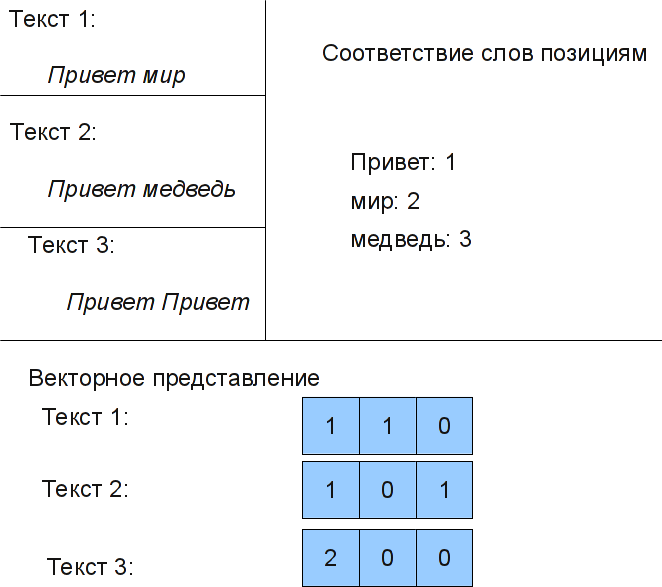
\includegraphics[width=10cm]{img/vectorize}
\end{center}
\caption{Векторное представление текста}
\label{svm-kernel}
\end{figure}

Для того чтобы понять о чем письмо необходимо анализировать входящие в него слова.
Хорошей характеристикой текста являются частоты входящих в него слов.
Таким образом мы можем взять все слова в языке, посчитать количество каждого из них в письме
и получить вектор частот.

Проблема заключается в том, что размерность такого вектора черезмерно высока причем
почти все признаки в этом случае окажутся нулевыми. Русский язык содержит около 100000 слов, а с
учетом словоформ количество слов может превысить несколько миллион.

Скорость работы метода опорных векторов линейно зависит размерности пространства классифицируемых векторов.
Большая размерность вектора приведет к увеличению времени построения модели и времени классификации.
Кроме того метод склонен к переобучению при больших размерностях векторов. Поэтому необходимо каким-то образом ограничить количество используемых для классификации слов.

Для решения задачи выбора используемых для классификации была произведена серия экспериментов.
Были протестированы следующие способы отбора:
\begin{itemize}
\item Выбор наиболее частых слов
\item Выбор случайно отобранных слов
\item Выбор слов для которых разница между частотой появления в спаме и в легитимной почте максимальна
\end{itemize}

Экспериментальным путем было установленно что наилучшие результаты метод опорных векторов проявляет при использовании 1500 самых частых слов. При меньшем количестве информации слишком мало для классификации, при большем - начинают проявляться проблемы переобучения.


\subsection{Многопрофильность}
